\documentclass[UKenglish,usenames,dvipsnames,svgnames,table,aspectratio=169,mathserif]{beamer}

\mode<presentation> {

%\usetheme{default}
\usetheme{Madrid}

\setbeamertemplate{footline} % To remove the footer line in all slides uncomment this line

\setbeamertemplate{navigation symbols}{} % To remove the navigation symbols from the bottom of all slides uncomment this line
}

\usepackage{graphicx} % Allows including images
\usepackage{booktabs} % Allows the use of \toprule, \midrule and \bottomrule in tables
\usepackage{hyperref}
\usepackage{apacite}
\usepackage{babel}
\usepackage{fancyvrb}
\usepackage{color}
\usepackage{alltt}
\usepackage{listings}
\usepackage{framed}
\usepackage{courier}
\usepackage{minted}
\usepackage{epstopdf}
\usepackage{xifthen}
\usepackage[utf8]{inputenc}
\usepackage[T1]{fontenc}
\usepackage{textcomp}
\usepackage{gensymb}
\usepackage{svg}
\usepackage{pdfpages}
\usepackage{isodate}

\hypersetup{colorlinks=false}

\setbeamertemplate{bibliography entry title}{}
\setbeamertemplate{bibliography entry location}{}
\setbeamertemplate{bibliography entry note}{}
\setbeamertemplate{itemize items}[circle]
\setbeamertemplate{enumerate items}[circle]
\beamertemplatenavigationsymbolsempty
\setbeamertemplate{footline}{}


\newminted{haskell}{}
\newminted{scala}{}

\definecolor{g}{RGB}{0,100,0}
\newcommand{\highlight}[1]{\colorbox{yellow}{#1}}
\newcommand{\nega}[1]{\colorbox{yellow}{#1}}
\newcommand{\posi}[1]{\colorbox{green}{#1}}
\newcommand{\nl}{\vspace{\baselineskip}}
\newcommand{\pnl}{\pause \nl}

\graphicspath{{diagrams/}}

\newcommand{\textslide}[1]{{
\begin{frame}
\begin{center}

#1

\end{center}
\end{frame}
}}

\newcommand{\textslideleft}[1]{{
\begin{frame}

#1

\end{frame}
}}

\newcommand{\codeslide}[1]{{
\begin{frame}[fragile]
\begin{haskellcode}
#1
\end{haskellcode}
\end{frame}
}}

\newcommand{\scalaslide}[1]{{
\begin{frame}[fragile]
\begin{scalacode}
#1
\end{scalacode}
\end{frame}
}}

\newcommand{\imageslide}[2][1]{{
\begin{frame}\begin{center}
\includegraphics[scale=#1]{#2}
\end{center}\end{frame}
}}

\newcommand{\imageslideleft}[2][1]{{
\begin{frame}
\includegraphics[scale=#1]{#2}
\end{frame}
}}

\newcommand{\imagetextslide}[3][1]{{
\begin{frame}\begin{center}

{#3}

\includegraphics[scale=#1]{#2}
\end{center}\end{frame}
}}

\newcommand{\svgslide}[1]{{
\begin{frame}
\begin{center}
\includesvg{diagrams/#1}
\end{center}
\end{frame}
}}

\definecolor{bgc}{RGB}{255, 255, 255}
\setbeamercolor{background canvas}{bg=bgc}


%%----------------------------------------------------------------------------------------
%	TITLE PAGE
%----------------------------------------------------------------------------------------

\title[Comma Police]{Comma Police: The Design and Implementation of a CSV Library}
\titlegraphic{
\includegraphics[scale=0.2]{data61.eps}}
\author{George Wilson}
\institute[]
{
Data61/CSIRO\\
\medskip
\href{george.wilson@data61.csiro.au}{george.wilson@data61.csiro.au}
}

\selectlanguage{UKenglish}
\date{\printdate{2018-05-23}}

\begin{document}

\begin{frame}
\titlepage
\end{frame}

%%%%%
%%%%% Intro section
%%%%%

\textslide{\LARGE
  JSON \\
  YAML \\
  XML \\
  CSV \\
  PSV \\

% \nl

% \large
% Many of us write programs which need to deal with one or more of these formats
}

\textslide{
{\Huge sv}

\nl

\large
\{CSV, PSV, \ldots\} library for Haskell
}


\begin{frame}[fragile]
\begin{columns}
\column{0.5\textwidth}
CSV

\begin{itemize}
\item Very popular format for data science
\item Described {\it not standardised} by RFC 4180
\end{itemize}

\column{0.05\textwidth}
\column{0.4\textwidth}
\begin{block}{example.csv}
\begin{Verbatim}
"id","species","count"
1,"kangaroo",30
2,"kookaburra",460
3,"platypus",5
\end{Verbatim}

\end{block}
\end{columns}
\end{frame}


\begin{frame}
\centering \nl \nl \nl \nl \nl
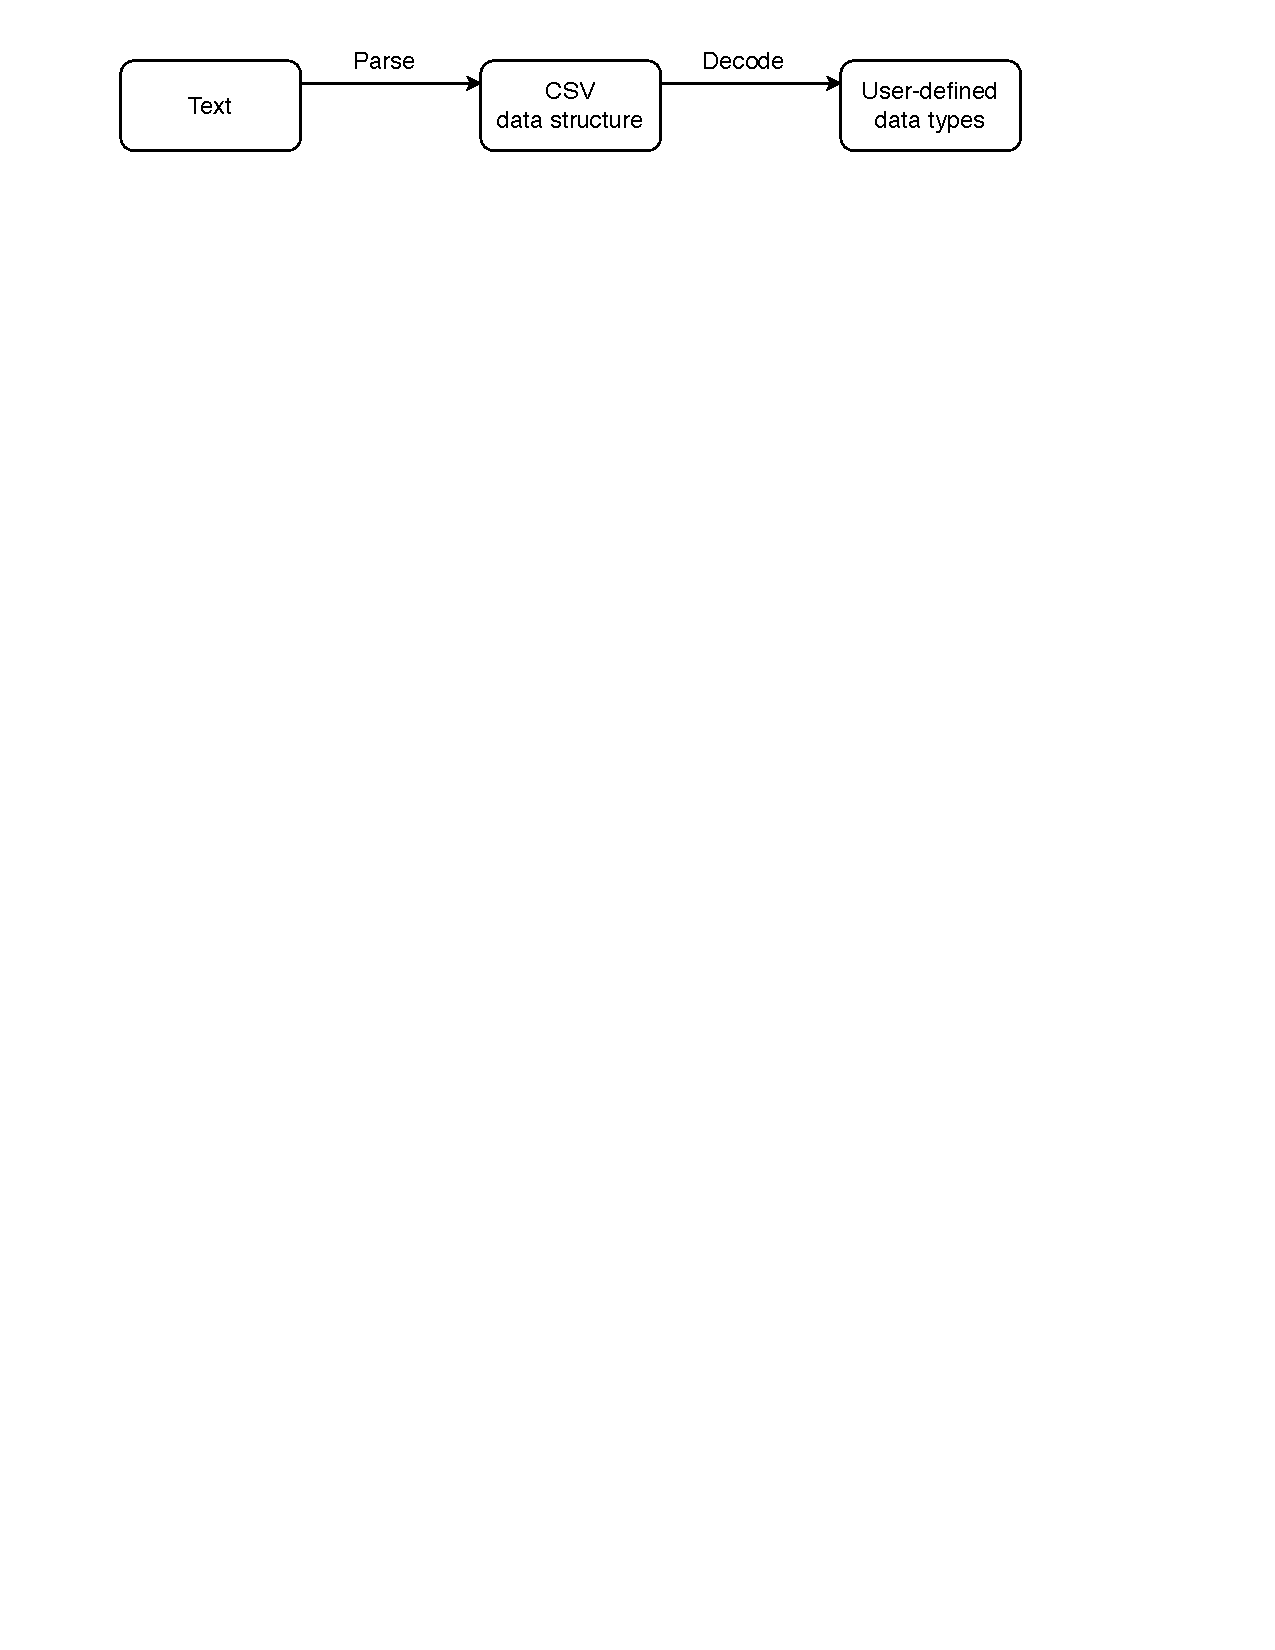
\includegraphics[scale=0.8]{diagrams/parsedecodeencodeprint1.pdf}
\end{frame}


\begin{frame}
\centering \nl \nl \nl \nl \nl
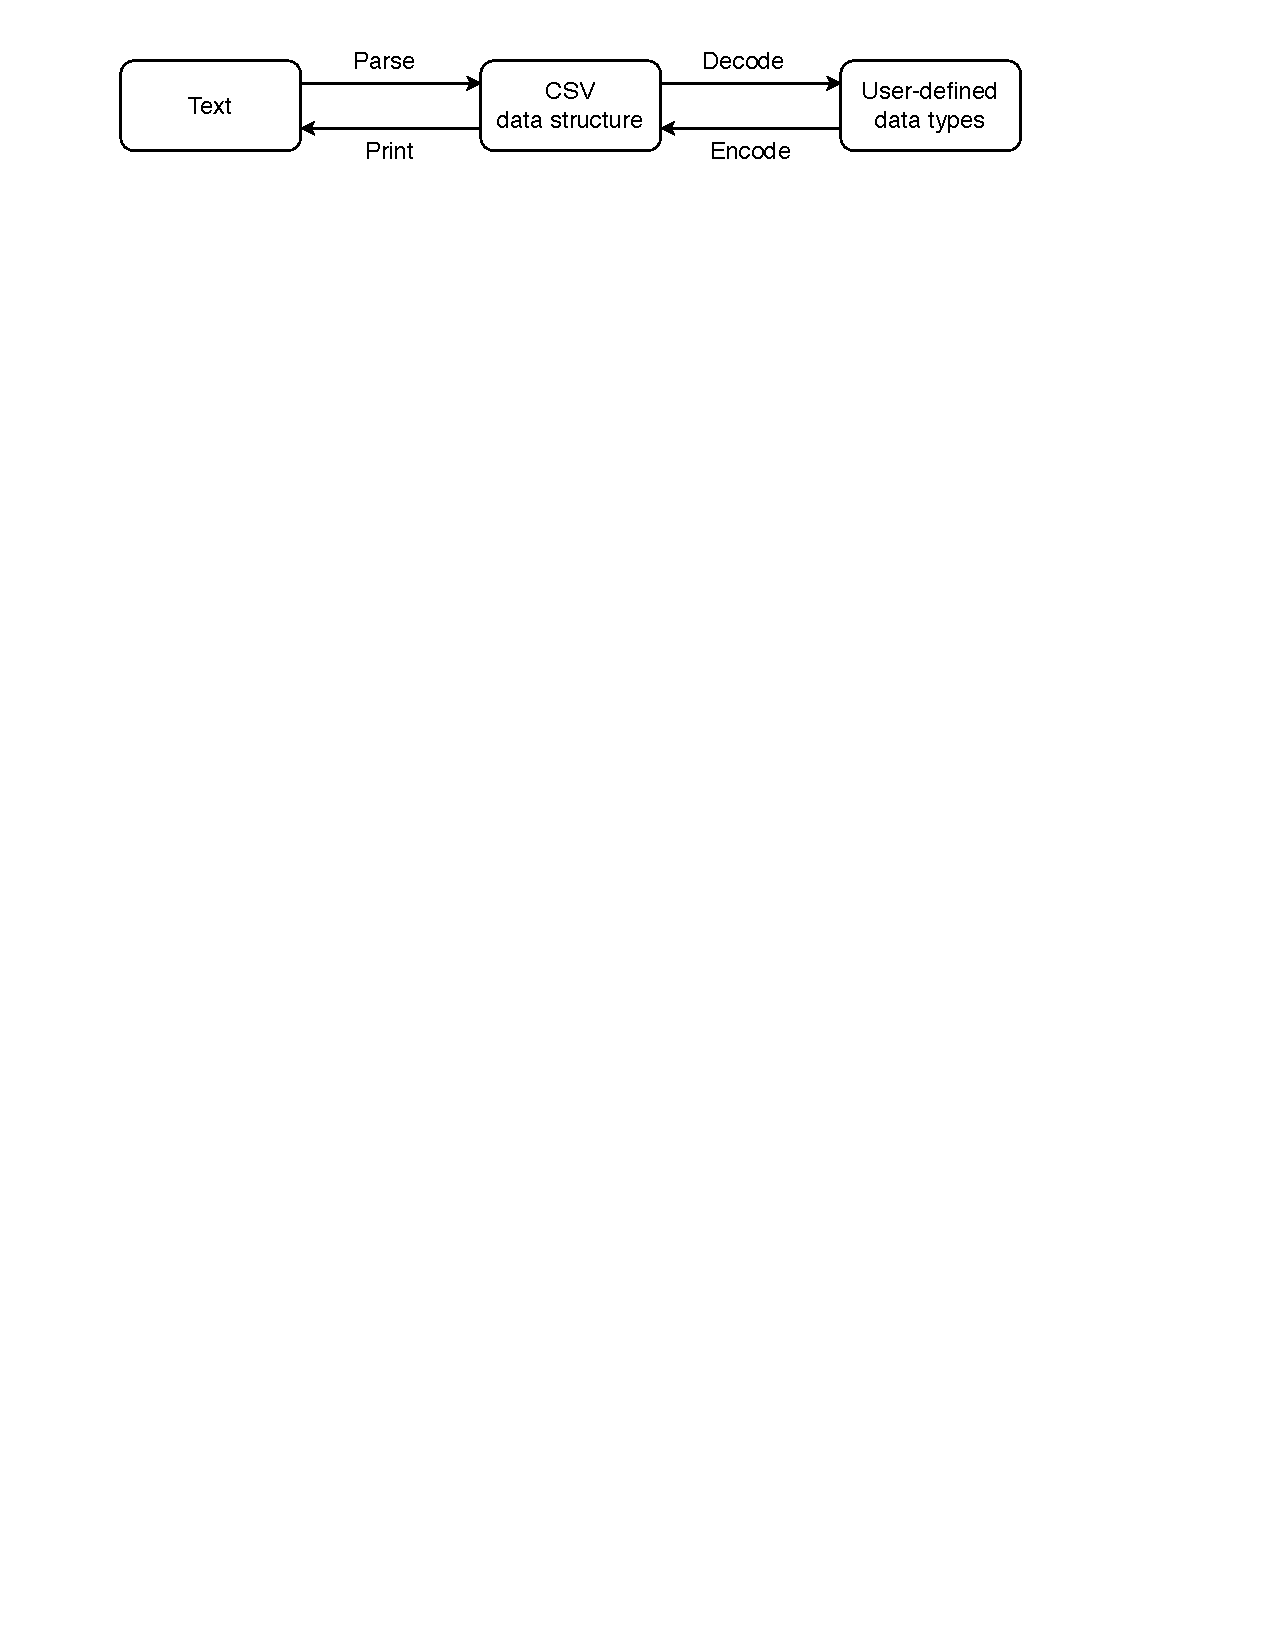
\includegraphics[scale=0.8]{diagrams/parsedecodeencodeprint2.pdf}
\end{frame}


\begin{frame}
\centering \nl \nl \nl \nl \nl
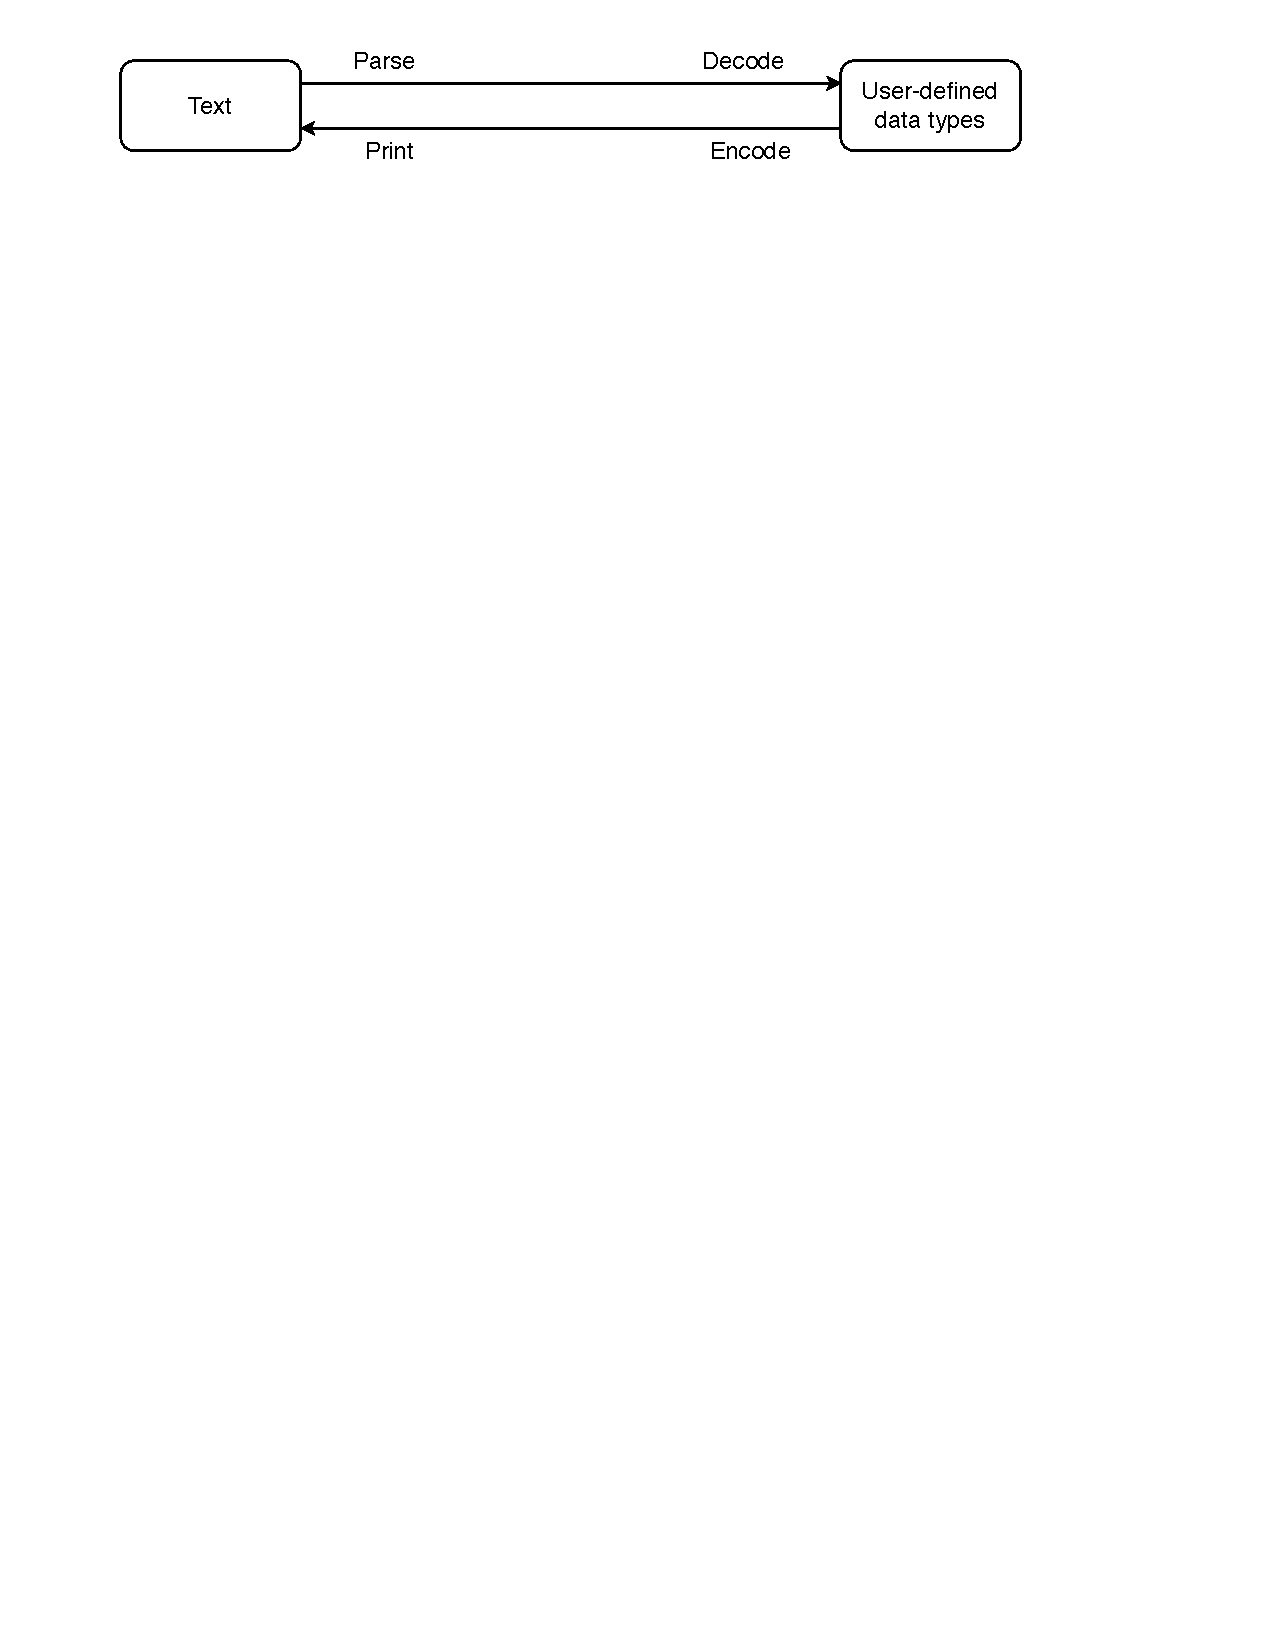
\includegraphics[scale=0.8]{diagrams/parsedecodeencodeprint3.pdf}
\end{frame}


\begin{frame}[fragile]
\begin{haskellcode}
parse :: ByteString -> Either ByteString (Sv ByteString)
\end{haskellcode}
\nl
\begin{haskellcode}
decode :: Decode s a -> Sv s -> DecodeValidation a
\end{haskellcode}
\nl
\begin{haskellcode}
encodeSv :: Encode a -> [a] -> Sv ByteString
\end{haskellcode}
\nl
\begin{haskellcode}
printSv :: Sv ByteString -> ByteString
\end{haskellcode}
\end{frame}


\begin{frame}
\begin{columns}
\column{0.3\textwidth}
{\bf Direct}
\begin{itemize}
\item less memory allocated
\item faster
\item streaming made easier
\end{itemize}

\column{0.5\textwidth}
{\bf Intermediate structure}

\begin{itemize}
\item potential for better errors (often)
\item make decisions based on the structure
\item manipulate the tree to alter documents
\end{itemize}
\end{columns}
\end{frame}


\begin{frame}
\begin{center}
%{\tt sv} keeps everything (including whitespace)
%\nl

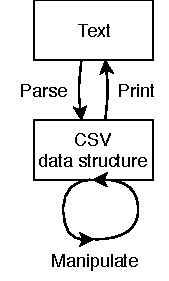
\includegraphics[scale=1.2]{pipeline-parse-print.pdf}
\end{center}
\end{frame}


% \begin{frame}
% \centering

% {\large sv provides lenses and traversals on its syntax tree}

% \nl

% \includegraphics[scale=0.3]{images/lens.jpg}

% \end{frame}

\begin{frame}[fragile]
\begin{block}{needs-fixing.csv}
\begin{Verbatim}
'name',"age"
"Frank",30
George, '25'
"Harry","32"
\end{Verbatim}
\end{block}
\end{frame}


\begin{frame}[fragile]
\begin{haskellcode}
fixQuotes :: Sv s -> Sv s
fixQuotes =
  over headerFields fixQuote . over recordFields fixQuote
    where
      headerFields = traverseHeader . fields
      recordFields = traverseRecords . fields

      fixQuote :: Field a -> Field a
      fixQuote f = case f of
        Unquoted a -> Quoted DoubleQuote (noEscape a)
        Quoted _ v -> Quoted DoubleQuote v
\end{haskellcode}
\end{frame}


\begin{frame}[fragile]
\begin{block}{needs-fixing.csv}
\begin{Verbatim}
'name',"age"
"Frank",30
George, '25'
"Harry","32"
\end{Verbatim}
\end{block}
\end{frame}


\begin{frame}[fragile]
\begin{block}{fixed.csv}
\begin{Verbatim}
"name","age"
"Frank","30"
"George", "25"
"Harry","32"
\end{Verbatim}
\end{block}
\end{frame}


\begin{frame}
\Large \centering
Use {\tt sv} to define custom linters and sanitisers

\nl
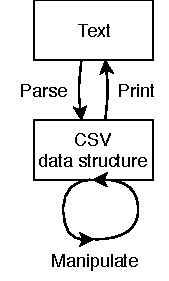
\includegraphics[scale=1]{pipeline-parse-print.pdf}

\end{frame}


\begin{frame}
\centering
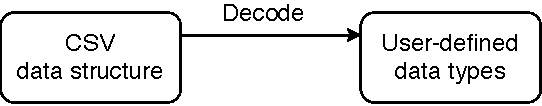
\includegraphics{decode.pdf}
\end{frame}


\begin{frame}[fragile]

% In sv, decoders are built from primitives and combinators

\begin{haskellcode}
data Decode s a = ...
\end{haskellcode}
\pnl
\begin{haskellcode}
raw    :: Decode a a
ignore :: Decode a ()
int    :: Decode ByteString Int
ascii  :: Decode ByteString String
text   :: Decode ByteString Text
\end{haskellcode}
\pnl
\begin{haskellcode}
instance Functor (Decode s)
instance Applicative (Decode s)
instance Alt (Decode s) where
\end{haskellcode}
\end{frame}


\begin{frame}[fragile]

\begin{block}{person.csv}
\begin{Verbatim}
"name","age"
"Frank","30"
"George", "25"
"Harry","32"
\end{Verbatim}
\end{block}

\pnl
\begin{haskellcode}
data Person = Person Text Int
\end{haskellcode}

\pnl

\begin{haskellcode}
personD :: Decode ByteString Person
personD = Person <$> text <*> int
\end{haskellcode}
\end{frame}


\begin{frame}[fragile]

\begin{block}{ragged.csv}
\begin{Verbatim}
"George","Wilson",25
"Frank",33
"Tim",18
"John","Smith",45
\end{Verbatim}
\end{block}

\pnl
\begin{haskellcode}
data Person
  = OneName Text Int
  | TwoNames Text Text Int
\end{haskellcode}

\pnl
\begin{haskellcode}
personDecoder :: Decode Person
personDecoder =
      OneName <$> text <*> int
  <!> TwoNames <$> text <*> text <*> int
\end{haskellcode}
\end{frame}


\begin{frame}[fragile]
\begin{haskellcode}
class Profunctor p where
  dimap :: (a -> b) -> (c -> d) -> p b c -> p a d

instance Profunctor Decode
\end{haskellcode}
\pnl
\begin{haskellcode}
-- make a Decode work on a different string type
decoder :: Decode ByteString A
input :: Text
\end{haskellcode}
\pause
\begin{haskellcode}
encodeUtf8 :: Text -> ByteString
\end{haskellcode}
\pause
\begin{haskellcode}
dimap encodeUtf8 id decoder :: Decode Text A
\end{haskellcode}
\end{frame}


\begin{frame}

{\Large Why not a type class?}


\begin{itemize}
\item A decoder is something I want to {\it manipulate}
\item There are often many different ways to decode the same type
\end{itemize}

\end{frame}


\begin{frame}[fragile]
\begin{haskellcode}
ignoreFailure :: Decode s a -> Decode s (Maybe a)
ignoreFailure a =
      Just <$> a
  <!> Nothing <* ignore
\end{haskellcode}

\pnl

\begin{block}{ints.csv}
\begin{Verbatim}
3
4
8.8
1
null
\end{Verbatim}
\end{block}

\pnl
\begin{haskellcode}
parseDecodefromFile (ignoreFailure int) "ints.csv"

-- [Just 3, Just 4, Nothing, Just 1, Nothing]
\end{haskellcode}

\end{frame}


\begin{frame}[fragile]

\begin{haskellcode}
-- succeeds with Nothing when
-- the underlying decoder fails
ignoreFailure :: Decode s a -> Decode s (Maybe a)

-- succeeds with Nothing only when
-- the field is completely empty
orEmpty :: Decode s a -> Decode s (Maybe a)

-- succeeds with Nothing only when
-- there is no field at all
optionalField :: Decode s a -> Decode s (Maybe a)
\end{haskellcode}

\end{frame}


%%%% TT SECTION
\begin{frame}[fragile]

\begin{block}{conferences.csv}
\begin{Verbatim}
"name","date"
"Compose Conf",20170828
"Compose Conf",20180827
"Lambda Jam",20170508
"Lambda Jam",20180521
\end{Verbatim}
\end{block}

\end{frame}


\begin{frame}[fragile]
\begin{haskellcode}
import Data.Thyme

data Conference = Conf Text YearMonthDay
\end{haskellcode}

\pnl
\begin{haskellcode}
ymdParser :: A.Parser YearMonthDay
ymdParser = buildTime <$> timeParser defaultTimeLocale "%Y%m%d"
\end{haskellcode}

\pnl
\begin{haskellcode}
trifecta   :: T.Parser a -> Decode ByteString a
attoparsec :: A.Parser a -> Decode ByteString a
\end{haskellcode}

\pnl
\begin{haskellcode}
ymd :: Decode YearMonthDay
ymd = attoparsec ymdParser
\end{haskellcode}
\pause
\begin{haskellcode}
confD :: Decode ByteString Conference
confD = Conf <$> text <*> ymd
\end{haskellcode}
\end{frame}


\begin{frame}[fragile]

{\tt sv} uses error values

\nl

\begin{haskellcode}
data DecodeError s
  = UnexpectedEndOfRow
  | ExpectedEndOfRow [Field s]
  | BadParse s
  | BadDecode s
  ...
\end{haskellcode}

\end{frame}


\begin{frame}[fragile]
\begin{haskellcode}
onError :: Decode s a
        -> (DecodeErrors s -> Decode s a)
        -> Decode s a
\end{haskellcode}
\end{frame}


\begin{frame}[fragile]
Rather than {\tt Either} for errors, sv uses the {\tt Validation} data type

\nl

\begin{haskellcode}
data Validation e a = Failure e | Success a
\end{haskellcode}

\pnl

\begin{haskellcode}
instance Semigroup e => Applicative (Validation e)
\end{haskellcode}

\pnl

\begin{haskellcode}
newtype DecodeErrors s =
  DecodeErrors (NonEmpty (DecodeError s))
  deriving Semigroup
\end{haskellcode}
\end{frame}


\begin{frame}[fragile]
\begin{block}{example.csv}
\begin{haskellcode}
"a","b","c"
\end{haskellcode}
\end{block}
\pnl
\begin{haskellcode}
data Two = Two Int Int
\end{haskellcode}
\pnl
\begin{haskellcode}
twoD :: Decode ByteString Two
twoD = Two <$> int <*> int
\end{haskellcode}
\pnl
\begin{haskellcode}
parseDecodeFromFile twoD "example.csv"
\end{haskellcode}
\pnl

\begin{block}

\begin{haskellcode}
Failure (DecodeErrors (
    BadDecode "Couldn't parse \"a\" as an int" :|
  [ BadDecode "Couldn't parse \"b\" as an int"
  , ExpectedEndOfRow ["c"]
  ]
))
\end{haskellcode}
\end{block}
\end{frame}


\begin{frame}
\Large \centering

What about encoding?

\nl
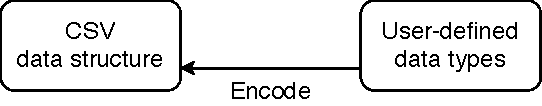
\includegraphics{encode.pdf}
\end{frame}


\begin{frame}[fragile]
\begin{haskellcode}
data Encode a = ...
\end{haskellcode}
\pnl
\begin{haskellcode}
int    :: Encode Int
double :: Encode Double
string :: Encode String
const  :: ByteString -> Encode a
encodeOf :: Prism' s a -> Encode a -> Encode s
\end{haskellcode}
\pnl
\begin{haskellcode}
instance Semigroup     (Encode a)

instance Contravariant  Encode
instance Divisible      Encode
instance Decidable      Encode
\end{haskellcode}
\end{frame}


\begin{frame}
\Huge \centering
Is it fast?

\pnl
No
\end{frame}


\begin{frame}

Benchmarks
\begin{itemize}
\item Benchmarked with a 100,000 line
\item Text, ints, doubles, products, sums
\item cassava vs. sv (instantiated to attoparsec)
\end{itemize}
\end{frame}


\begin{frame}
\centering
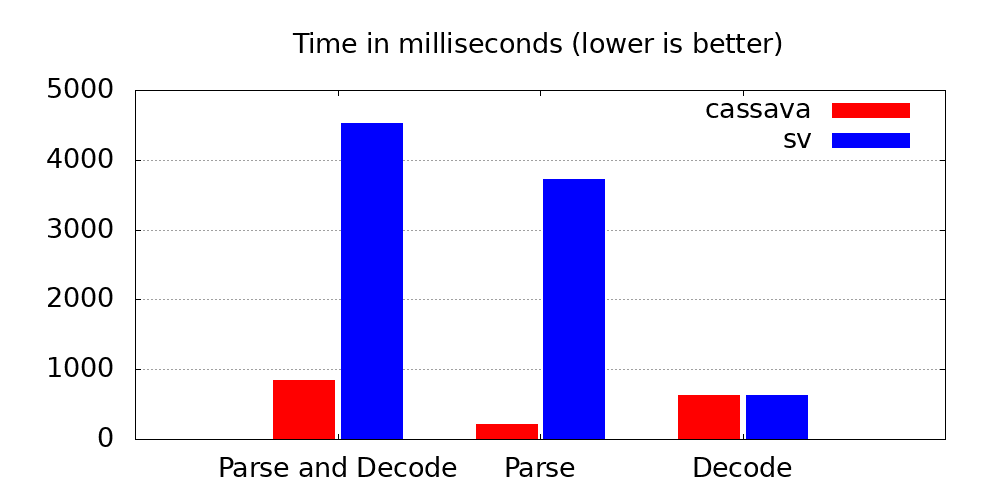
\includegraphics[scale=0.5]{data/bench.png}

\pnl

Use {\tt sv-cassava} for now
\end{frame}


\begin{frame}

{\bf Noteworthy limitations as at 2018-05-23}

\begin{itemize}
\item No column-name-based decoding
\item Errors don't report source-file positions
\item No streaming
\item Performance needs work (particularly in parsing)
\end{itemize}
\end{frame}


\textslide{{\Large

Contributions to sv are welcome.

\nl

Do you have a crazy CSV file to challenge sv?

\nl

Contact me at \href{mailto:george.wilson@data61.csiro.au}{george.wilson@data61.csiro.au}
}}


\textslide{
{\huge References}

\begin{itemize}
\item {\tt sv} library \\
  \url{https://github.com/qfpl/sv} \\
  \url{https://github.com/qfpl/sv-cassava}
\item validation data type \\
  \url{https://hackage.haskell.org/package/validation} \\
  \url{https://hackage.haskell.org/package/either}
\item CSV RFC \\
  \url{https://tools.ietf.org/html/rfc4180}
\item Hedgehog \\
  \url{https://hackage.haskell.org/package/hedgehog}
\end{itemize}
}

\textslide{\Huge Thanks for listening!}



\end{document}

